\documentclass[11pt]{article}
\usepackage[a4paper,margin=0.85in]{geometry}
\usepackage{graphicx}
\usepackage{amsmath,amssymb}
\usepackage{booktabs}
\usepackage{tabularx}
\usepackage{array}
\usepackage{hyperref}
\usepackage{caption}
\usepackage{xcolor}
\usepackage{enumitem}
\setlist[itemize]{leftmargin=1.2em}
\setlist[enumerate]{leftmargin=1.4em}

\title{Mechanism Graphs for the LHC Black-Hole Safety Case}
\author{Static audit report}
\date{}

\begin{document}
\maketitle

\begin{abstract}
Scientific papers contain an attribution layer and an equation layer. The first records
sources and claims. The second records the mathematical steps that could make a claim
physically true. This report applies that separation to the LHC microscopic-black-hole
safety debate using a static public audit run. The selected corpus contains
492 arXiv sources, 377
provenance claim nodes and 1,408 equation witnesses.
Formula gates reduce the equation layer to 204
usable mechanism nodes and 35
evidence-grade case nodes. The branch split is sharp:
0 source-local formula-clean
direct LHC-safety mechanisms, 1
collider-threshold hook and 28
astrophysical black-hole analogues. The useful object is a translation map: accretion,
evaporation, capture, mass growth and compact-object survival mechanisms must be carried
explicitly into the collider branch before they can support a safety argument.
\end{abstract}

\section{Main Claims and Evidence Register}

\begin{enumerate}
\item \textbf{The selected corpus supports a selected-corpus finding.} Evidence: 492 selected sources from the high-recall scan. Interpretation: The scan is broad enough for this public audit object. A universal absence claim would require the full literature and non-arXiv safety reports.
\item \textbf{The provenance layer is mostly attribution.} Evidence: 869 provenance nodes and 377 source-to-claim edges. Interpretation: It organizes who said what and where. Equation support has to be tested in a separate graph.
\item \textbf{The mechanism layer is much stricter than the provenance layer.} Evidence: 1408 equation witnesses narrowed to 204 usable mechanism nodes. Interpretation: Most extracted text is retained as audit material or rejected by formula-quality gates.
\item \textbf{No direct LHC-safety equation branch passed the strict gate.} Evidence: 0 direct LHC-safety mechanism nodes. Interpretation: The absence is defined by the selected corpus and the source-local equation gate.
\item \textbf{The populated branch is adjacent black-hole physics.} Evidence: 28 astrophysical analogues and 1 collider-threshold hook. Interpretation: The audit becomes mechanism translation from accretion, evaporation, capture and compact-object survival into the collider branch.
\item \textbf{The dominant mechanism routes are operator/closure/transport.} Evidence: constraint closure=165, spectral operator=160, transport flow=95 Interpretation: The graph records equation roles and route co-activation.
\item \textbf{Sparse attention supports the branch split.} Evidence: spectral operator=34, constraint closure=33, transport flow=25 Interpretation: The sparse audit is a consistency check over static graph artifacts.
\end{enumerate}

\section{Data Object}

The run directory is \texttt{runs/lhc\_black\_hole\_audit\_500k\_strict}. It contains derived public artifacts:
\texttt{manifest.json}, \texttt{provenance\_graph.json}, \texttt{equation\_witnesses.json},
\texttt{operational\_graph.json}, \texttt{equation\_mechanism\_graph.json} and
\texttt{sparse\_attention\_audit.json}. These files are enough to inspect the report. Private
fingerprints, model checkpoints and core pipeline files are outside this repository.

\begin{figure}[t]
\centering
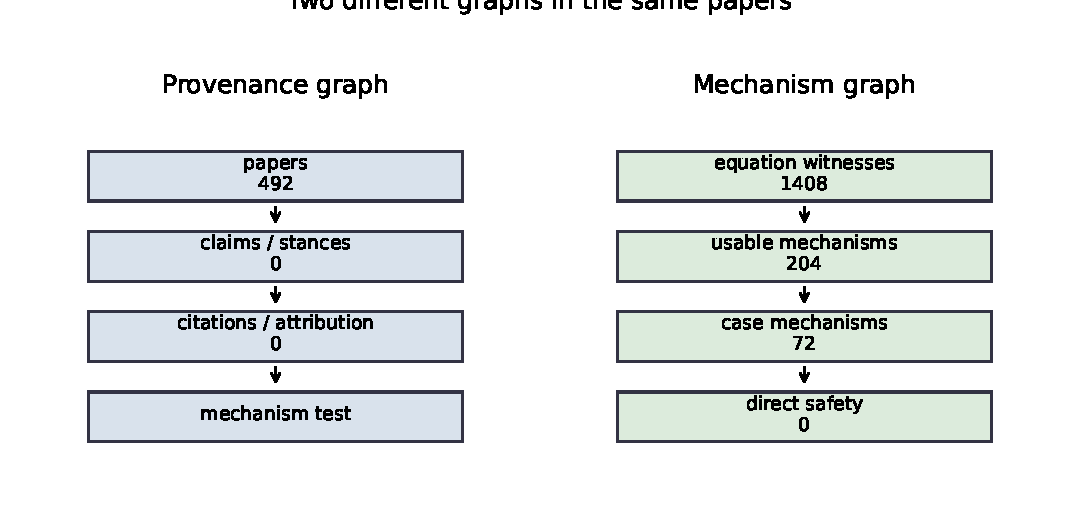
\includegraphics[width=0.92\linewidth]{figures/provenance_vs_mechanism.pdf}
\caption{Two graph layers in the same selected archive. Provenance organizes attribution and claims. The mechanism graph records which equation-level branches are present.}
\end{figure}

\section{Provenance Layer}

The provenance layer contains 869 nodes and
377 source-to-claim edges. Claim labels in this selected
corpus are:

\begin{center}
\begin{tabular}{lr}
\toprule
Quantity & Count\\
\midrule
astrophysical claim & 355\\
risk claim & 20\\
safety claim & 2\\
\bottomrule
\end{tabular}
\end{center}

\begin{figure}[t]
\centering
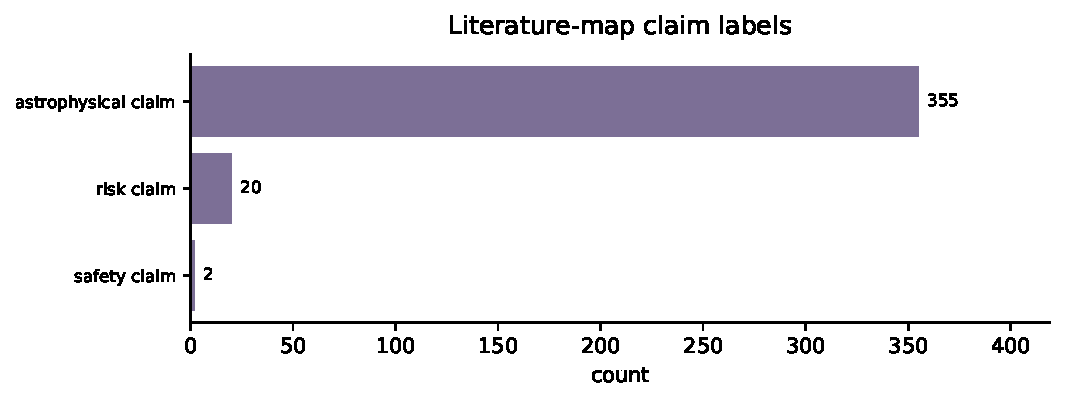
\includegraphics[width=0.74\linewidth]{figures/final_claim_types.pdf}
\caption{Claim labels in the provenance layer. This layer is an attribution record. Equation support is tested separately.}
\end{figure}

\section{Mechanism Layer and Gates}

The mechanism layer begins with local equation witnesses and applies formula-quality, case-relevance
and route gates. The public audit uses six route labels:
\[
\begin{array}{ll}
\text{transport/flow} & \partial_t q + \nabla\cdot J = S,\\
\text{constraint/closure} & C(q,J,\lambda)=0,\\
\text{spectral/operator} & Lq=\lambda q,\\
\text{boundary/weak form} & \int_\Omega \phi Lq=\int_\Omega \phi f,\quad Bq=b,\\
\text{commutator/residual} & [A,B]=AB-BA,\\
\text{discrete protocol} & x_{n+1}=\Phi(x_n,u_n).
\end{array}
\]
These route labels are audit gates. They separate formula-clean mechanism receipts from word
matches and bibliographic residue.

\begin{figure}[t]
\centering
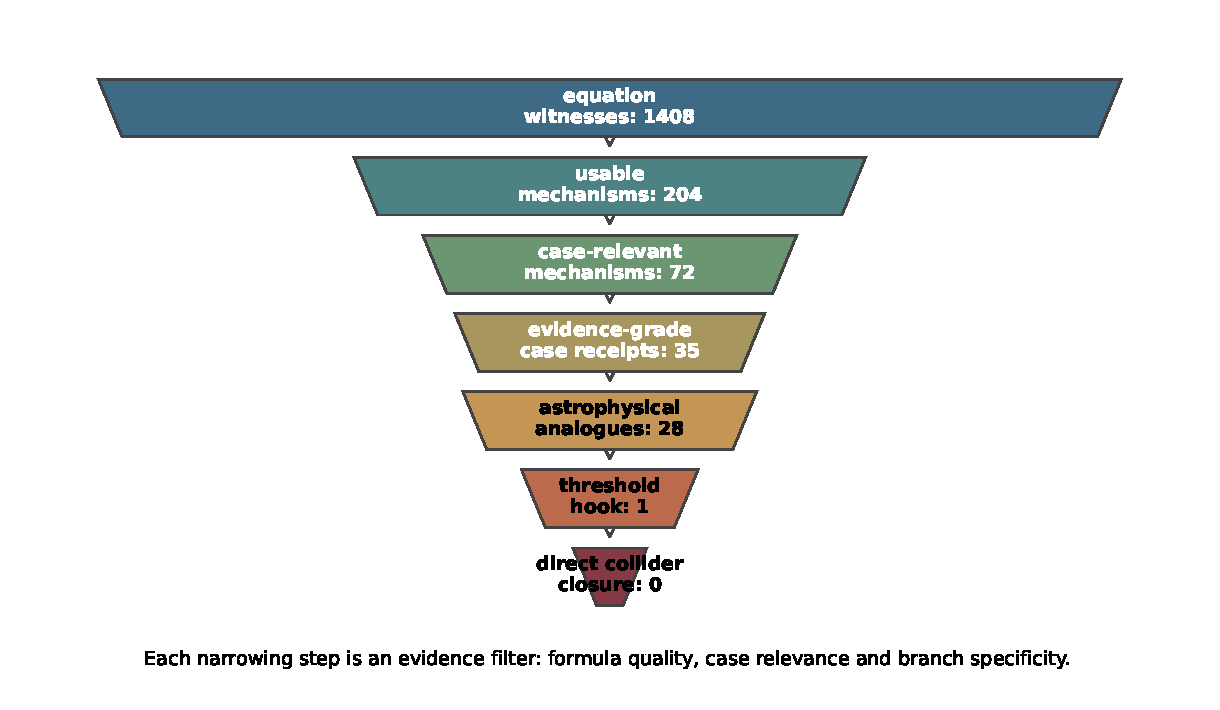
\includegraphics[width=0.82\linewidth]{figures/final_evidence_funnel.pdf}
\caption{Strict evidence funnel from equation witnesses to case-specific mechanism receipts. The sharp drop is expected: the gate rejects prose fragments, local word matches without a relation operator, and formula windows without case-local mechanism content.}
\end{figure}

\section{Run Counts}

\begin{center}
\begin{tabular}{lr}
\toprule
Quantity & Count\\
\midrule
selected sources & 492\\
provenance claims & 377\\
source equation witnesses & 1,408\\
usable mechanism nodes & 204\\
case-relevant mechanism nodes & 72\\
evidence-grade case nodes & 35\\
direct LHC-safety mechanism nodes & 0\\
collider-threshold hooks & 1\\
astrophysical analogues & 28\\
source-local route-transition edges & 120\\
rich cross-source route analogues & 130\\
\bottomrule
\end{tabular}
\end{center}

\section{Mechanism Distribution}

The usable mechanism layer is dominated by closure, spectral/operator and transport routes:

\begin{center}
\begin{tabular}{lr}
\toprule
Quantity & Count\\
\midrule
constraint closure & 165\\
spectral operator & 160\\
transport flow & 95\\
boundary weak form & 28\\
discrete protocol & 24\\
commutator incompatibility & 12\\
\bottomrule
\end{tabular}
\end{center}

\begin{figure}[t]
\centering
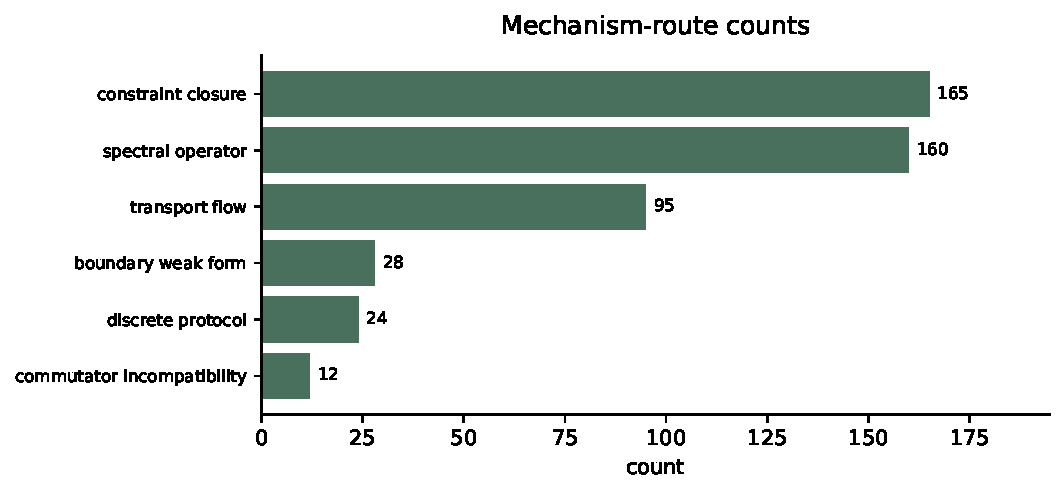
\includegraphics[width=0.82\linewidth]{figures/final_route_counts.pdf}
\caption{Six-route counts among non-artifact constructor pairs. The reusable layer is a small set of equation operations.}
\end{figure}

Constructor-role and transition-label diagnostics give the same picture:

\begin{center}
\begin{tabular}{lr}
\toprule
Quantity & Count\\
\midrule
operator apparatus & 142\\
selector & 106\\
real substrate geometry & 94\\
closure constraints & 68\\
readout current & 45\\
protocol order & 25\\
\bottomrule
\end{tabular}
\end{center}

\begin{figure}[t]
\centering
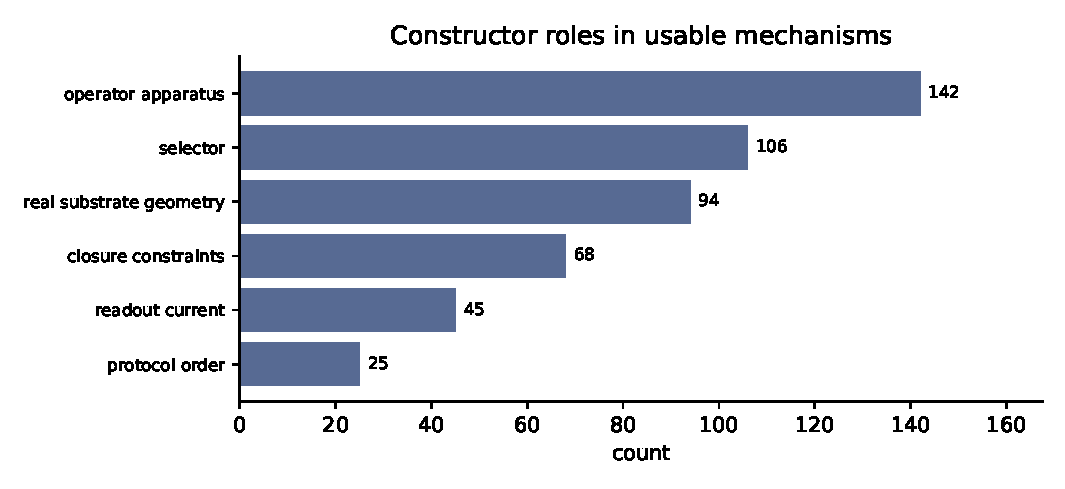
\includegraphics[width=0.82\linewidth]{figures/final_constructor_roles.pdf}
\caption{Constructor roles present in usable mechanisms. Operator apparatus, selector and real substrate geometry appear as separable roles.}
\end{figure}

\begin{figure}[t]
\centering
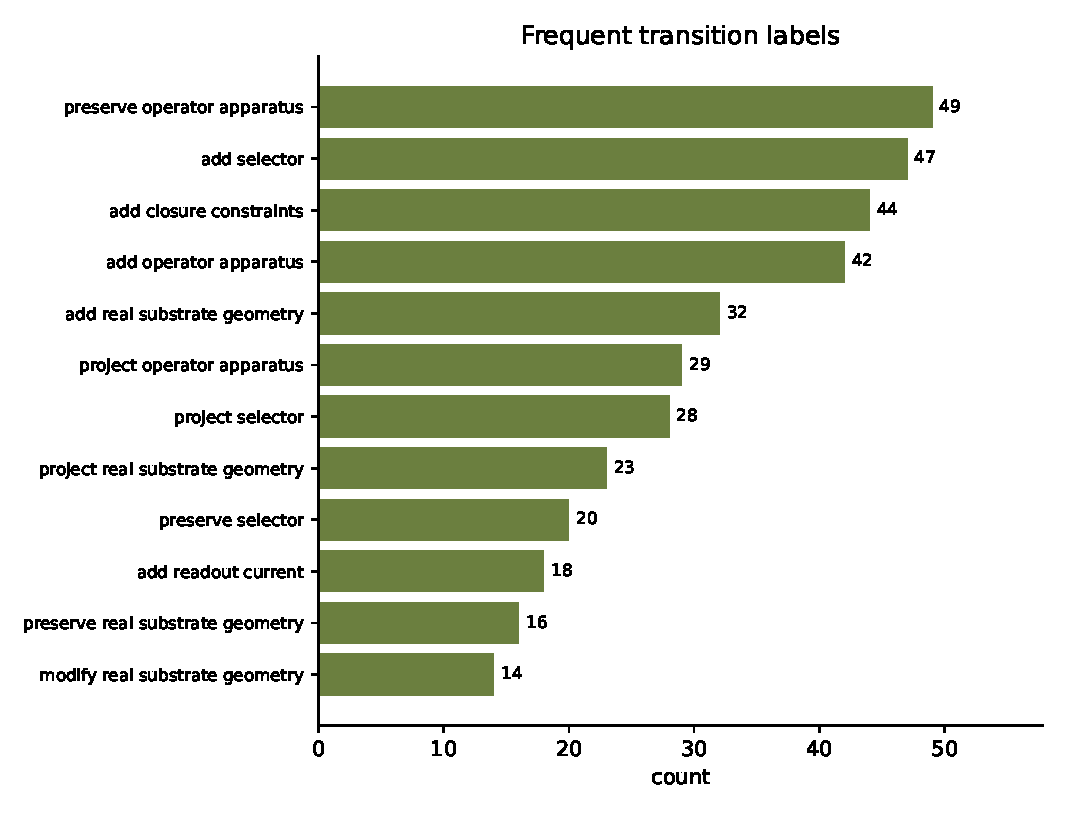
\includegraphics[width=0.86\linewidth]{figures/final_transition_labels.pdf}
\caption{Frequent transition labels. Preservation, addition and projection of operator, selector and closure roles are common moves in the equation layer.}
\end{figure}

\section{LHC Case Branches}

Evidence-grade branch counts are:

\begin{center}
\begin{tabular}{lr}
\toprule
Quantity & Count\\
\midrule
stable growth or capture branch & 29\\
astrophysical black hole analogue & 28\\
evaporation branch & 12\\
production threshold branch & 1\\
\bottomrule
\end{tabular}
\end{center}

\begin{figure}[t]
\centering
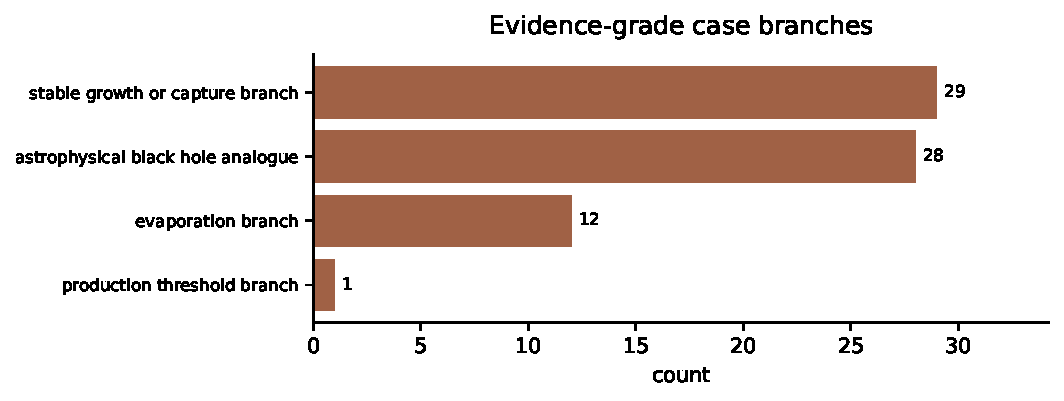
\includegraphics[width=0.82\linewidth]{figures/final_case_branches.pdf}
\caption{Evidence-grade case branches. The populated branch is adjacent astrophysical black-hole physics; the direct LHC-safety branch remains empty under the strict gate.}
\end{figure}

The collider branch first requires a production or event-selection condition, for example
\[
\sqrt{s} > M_D .
\]
If evaporation dominates, a local receipt should support a mass-loss or lifetime ordering such as
\[
\frac{dM}{dt} < 0,\qquad \tau_{\rm evap}\ll \tau_{\rm capture} .
\]
If a stable object is assumed, the mechanism changes to stopping, capture and growth:
\[
\frac{dM}{dt}=\rho\,\sigma(M)\,v .
\]
Compact-object survival then becomes an external constraint on the same mechanism:
\[
t_{\rm grow} < t_{\rm WD}
\]
would be inconsistent with observed white-dwarf survival if the same production, capture and
growth mechanism were realized in nature. The static graph found adjacent receipts for this
translation problem. It did not find a direct formula-clean collider-safety branch.

\section{Sparse-Attention Check}

The sparse-attention audit reads the static mechanism graph and measures route co-activation in
the evidence-grade case layer.

\begin{itemize}
\item Evidence-grade routes: spectral operator=34, constraint closure=33, transport flow=25, boundary weak form=4.
\item Astrophysical analogues concentrate on spectral operator=0.35, constraint closure=0.34, transport flow=0.26, boundary weak form=0.04.
\item The production-threshold branch is small and separate: boundary weak form=0.50, constraint closure=0.50.
\item The strongest route co-activations are constraint closure + spectral operator=32, spectral operator + transport flow=25, constraint closure + transport flow=23.
\end{itemize}

\begin{figure}[t]
\centering
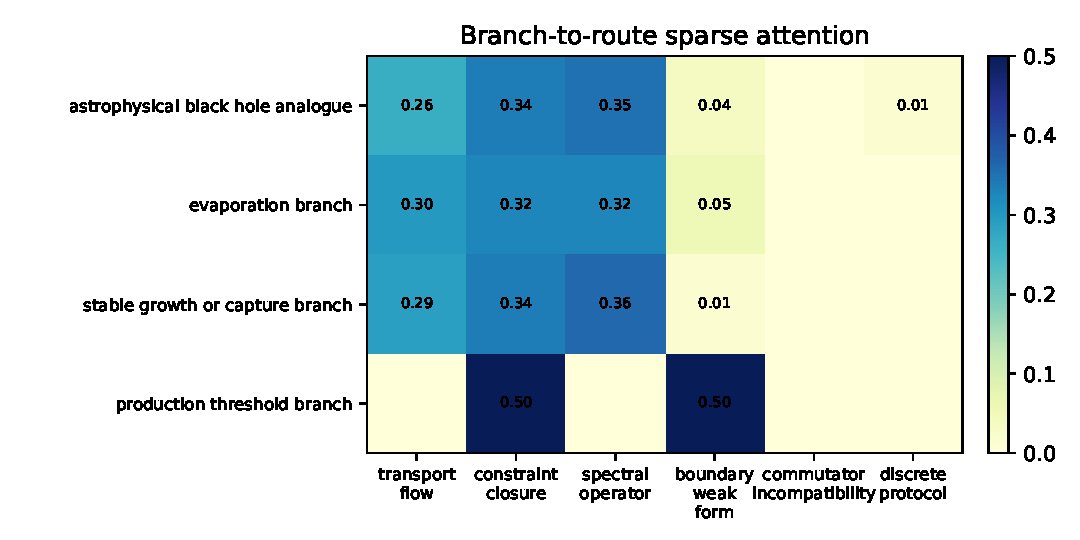
\includegraphics[width=0.88\linewidth]{figures/final_sparse_attention.pdf}
\caption{Branch-to-route sparse attention. Astrophysical analogues activate operator, closure and transport routes; the production-threshold branch is separated.}
\end{figure}

\section{Equation Receipts}

\subsection{Direct LHC-Safety Receipts}
\emph{No receipt passed the current gate.}

\subsection{Collider-Threshold or Event-Selection Hook}
\begin{tabularx}{\linewidth}{p{0.14\linewidth}p{0.23\linewidth}p{0.24\linewidth}X}
\toprule
Source & Routes & Branch labels & Formula witness\\
\midrule
0904.0230 / E00053 & constraint closure, boundary weak form & production threshold branch & \begin{minipage}[t]{\linewidth}\raggedright\scriptsize\ttfamily |y\_\{\textbackslash{}gamma \textbackslash{}gamma\}| \textbackslash{}leq 1\end{minipage}\tabularnewline
\bottomrule
\end{tabularx}

\subsection{Astrophysical Black-Hole Analogues}
\begin{tabularx}{\linewidth}{p{0.14\linewidth}p{0.23\linewidth}p{0.24\linewidth}X}
\toprule
Source & Routes & Branch labels & Formula witness\\
\midrule
0807.3458 / E00034 & transport flow, constraint closure, spectral operator & astrophysical black hole analogue, evaporation branch, stable growth or capture branch & \begin{minipage}[t]{\linewidth}\raggedright\scriptsize\ttfamily 3 \textbackslash{}times 10\textasciicircum{}\{-13\}\textasciitilde{}\textbackslash{}mathrm\{M\}\\ \_\{\textbackslash{}odot\}\textasciitilde{}\textbackslash{}mathrm\{yr\}\textasciicircum{}\{-1\}\\ \textbackslash{}lesssim \textbackslash{}langle\\ \textbackslash{}dot\{M\}\_\{\textbackslash{}mathrm\{long\}\}\\ \textbackslash{}rangle \textbackslash{}lesssim 1 \textbackslash{}times 10\\ \textasciicircum{}\{-10\}\textasciitilde{}\textbackslash{}mathrm\{M\}\_\{\textbackslash{}odot\}\textasciitilde{}..\\ .\end{minipage}\tabularnewline
0807.3458 / E00035 & transport flow, constraint closure, spectral operator & astrophysical black hole analogue, evaporation branch, stable growth or capture branch & \begin{minipage}[t]{\linewidth}\raggedright\scriptsize\ttfamily 4 \textbackslash{}times 10\textasciicircum{}\{-14\}\textasciitilde{}\textbackslash{}mathrm\{M\}\\ \_\{\textbackslash{}odot\}\textasciitilde{}\textbackslash{}mathrm\{yr\}\textasciicircum{}\{-1\}\\ \textbackslash{}lesssim \textbackslash{}langle\\ \textbackslash{}dot\{M\}\_\{\textbackslash{}mathrm\{long\}\}\\ \textbackslash{}rangle \textbackslash{}lesssim 2 \textbackslash{}times 10\\ \textasciicircum{}\{-11\}\textasciitilde{}\textbackslash{}mathrm\{M\}\_\{\textbackslash{}odot\}\textasciitilde{}..\\ .\end{minipage}\tabularnewline
astro-ph0212297 / E01142 & constraint closure, transport flow, spectral operator & astrophysical black hole analogue, evaporation branch, stable growth or capture branch & \begin{minipage}[t]{\linewidth}\raggedright\scriptsize\ttfamily B\_c\textbackslash{}simeq 10\textasciicircum{}\{16\}\textbackslash{}mbox\{G\}\textbackslash{}le\\ ft(\{7M\_\textbackslash{}odot\}/\{M\_H\}\textbackslash{}right) \textbackslash{}\\ left(\{6M\_H\}/\{R\}\textbackslash{}right)\textasciicircum{}2\textbackslash{}lef\\ t(\{M\_T\}/\{0.03M\_H\}\textbackslash{}right)\textasciicircum{}\{1/\\ 2\}\end{minipage}\tabularnewline
1307.7685 / E00825 & constraint closure, transport flow, spectral operator & astrophysical black hole analogue, stable growth or capture branch & \begin{minipage}[t]{\linewidth}\raggedright\scriptsize\ttfamily \textbackslash{}delta M\_\{BH\}< 5 \textbackslash{}times\\ 10\textasciicircum{}\{-4\}M\_\{BH\}\end{minipage}\tabularnewline
1207.1244 / E00797 & constraint closure, transport flow, spectral operator, discrete protocol & astrophysical black hole analogue & \begin{minipage}[t]{\linewidth}\raggedright\scriptsize\ttfamily M\_1 = 0.9\_\{-0.3\}\textasciicircum{}\{+4.6\}\\ M\_\textbackslash{}odot\end{minipage}\tabularnewline
1604.02455 / E01020 & constraint closure, transport flow, spectral operator & astrophysical black hole analogue, evaporation branch, stable growth or capture branch & \begin{minipage}[t]{\linewidth}\raggedright\scriptsize\ttfamily 4000M \textbackslash{}sim 60(M\_\{\textbackslash{}rm\\ NS/1.625M\_\textbackslash{}odot)\end{minipage}\tabularnewline
1604.02455 / E01021 & constraint closure, transport flow, spectral operator & astrophysical black hole analogue, evaporation branch, stable growth or capture branch & \begin{minipage}[t]{\linewidth}\raggedright\scriptsize\ttfamily \textbackslash{}Delta t \textbackslash{}sim 0.1 (M\_\{\textbackslash{}rm\\ NS/1.625M\_\textbackslash{}odot)\end{minipage}\tabularnewline
astro-ph0212297 / E01141 & constraint closure, spectral operator, transport flow & astrophysical black hole analogue, evaporation branch, stable growth or capture branch & \begin{minipage}[t]{\linewidth}\raggedright\scriptsize\ttfamily \{\textbackslash{}cal E\_B\}/\{\{\textbackslash{}cal E\}\_k\}<0.1\end{minipage}\tabularnewline
\bottomrule
\end{tabularx}

\subsection{Stable Growth or Capture Branch}
\begin{tabularx}{\linewidth}{p{0.14\linewidth}p{0.23\linewidth}p{0.24\linewidth}X}
\toprule
Source & Routes & Branch labels & Formula witness\\
\midrule
0807.3458 / E00034 & transport flow, constraint closure, spectral operator & astrophysical black hole analogue, evaporation branch, stable growth or capture branch & \begin{minipage}[t]{\linewidth}\raggedright\scriptsize\ttfamily 3 \textbackslash{}times 10\textasciicircum{}\{-13\}\textasciitilde{}\textbackslash{}mathrm\{M\}\\ \_\{\textbackslash{}odot\}\textasciitilde{}\textbackslash{}mathrm\{yr\}\textasciicircum{}\{-1\}\\ \textbackslash{}lesssim \textbackslash{}langle\\ \textbackslash{}dot\{M\}\_\{\textbackslash{}mathrm\{long\}\}\\ \textbackslash{}rangle \textbackslash{}lesssim 1 \textbackslash{}times 10\\ \textasciicircum{}\{-10\}\textasciitilde{}\textbackslash{}mathrm\{M\}\_\{\textbackslash{}odot\}\textasciitilde{}..\\ .\end{minipage}\tabularnewline
0807.3458 / E00035 & transport flow, constraint closure, spectral operator & astrophysical black hole analogue, evaporation branch, stable growth or capture branch & \begin{minipage}[t]{\linewidth}\raggedright\scriptsize\ttfamily 4 \textbackslash{}times 10\textasciicircum{}\{-14\}\textasciitilde{}\textbackslash{}mathrm\{M\}\\ \_\{\textbackslash{}odot\}\textasciitilde{}\textbackslash{}mathrm\{yr\}\textasciicircum{}\{-1\}\\ \textbackslash{}lesssim \textbackslash{}langle\\ \textbackslash{}dot\{M\}\_\{\textbackslash{}mathrm\{long\}\}\\ \textbackslash{}rangle \textbackslash{}lesssim 2 \textbackslash{}times 10\\ \textasciicircum{}\{-11\}\textasciitilde{}\textbackslash{}mathrm\{M\}\_\{\textbackslash{}odot\}\textasciitilde{}..\\ .\end{minipage}\tabularnewline
astro-ph0212297 / E01142 & constraint closure, transport flow, spectral operator & astrophysical black hole analogue, evaporation branch, stable growth or capture branch & \begin{minipage}[t]{\linewidth}\raggedright\scriptsize\ttfamily B\_c\textbackslash{}simeq 10\textasciicircum{}\{16\}\textbackslash{}mbox\{G\}\textbackslash{}le\\ ft(\{7M\_\textbackslash{}odot\}/\{M\_H\}\textbackslash{}right) \textbackslash{}\\ left(\{6M\_H\}/\{R\}\textbackslash{}right)\textasciicircum{}2\textbackslash{}lef\\ t(\{M\_T\}/\{0.03M\_H\}\textbackslash{}right)\textasciicircum{}\{1/\\ 2\}\end{minipage}\tabularnewline
astro-ph0109539 / E01098 & constraint closure, spectral operator, transport flow & stable growth or capture branch & \begin{minipage}[t]{\linewidth}\raggedright\scriptsize\ttfamily \textbackslash{}langle M\textbackslash{}rangle \textbackslash{}sim 9\\ \{M\}\_\textbackslash{}odot\end{minipage}\tabularnewline
1307.7685 / E00825 & constraint closure, transport flow, spectral operator & astrophysical black hole analogue, stable growth or capture branch & \begin{minipage}[t]{\linewidth}\raggedright\scriptsize\ttfamily \textbackslash{}delta M\_\{BH\}< 5 \textbackslash{}times\\ 10\textasciicircum{}\{-4\}M\_\{BH\}\end{minipage}\tabularnewline
1604.02455 / E01020 & constraint closure, transport flow, spectral operator & astrophysical black hole analogue, evaporation branch, stable growth or capture branch & \begin{minipage}[t]{\linewidth}\raggedright\scriptsize\ttfamily 4000M \textbackslash{}sim 60(M\_\{\textbackslash{}rm\\ NS/1.625M\_\textbackslash{}odot)\end{minipage}\tabularnewline
\bottomrule
\end{tabularx}

\subsection{Evaporation Branch}
\begin{tabularx}{\linewidth}{p{0.14\linewidth}p{0.23\linewidth}p{0.24\linewidth}X}
\toprule
Source & Routes & Branch labels & Formula witness\\
\midrule
0807.3458 / E00034 & transport flow, constraint closure, spectral operator & astrophysical black hole analogue, evaporation branch, stable growth or capture branch & \begin{minipage}[t]{\linewidth}\raggedright\scriptsize\ttfamily 3 \textbackslash{}times 10\textasciicircum{}\{-13\}\textasciitilde{}\textbackslash{}mathrm\{M\}\\ \_\{\textbackslash{}odot\}\textasciitilde{}\textbackslash{}mathrm\{yr\}\textasciicircum{}\{-1\}\\ \textbackslash{}lesssim \textbackslash{}langle\\ \textbackslash{}dot\{M\}\_\{\textbackslash{}mathrm\{long\}\}\\ \textbackslash{}rangle \textbackslash{}lesssim 1 \textbackslash{}times 10\\ \textasciicircum{}\{-10\}\textasciitilde{}\textbackslash{}mathrm\{M\}\_\{\textbackslash{}odot\}\textasciitilde{}..\\ .\end{minipage}\tabularnewline
0807.3458 / E00035 & transport flow, constraint closure, spectral operator & astrophysical black hole analogue, evaporation branch, stable growth or capture branch & \begin{minipage}[t]{\linewidth}\raggedright\scriptsize\ttfamily 4 \textbackslash{}times 10\textasciicircum{}\{-14\}\textasciitilde{}\textbackslash{}mathrm\{M\}\\ \_\{\textbackslash{}odot\}\textasciitilde{}\textbackslash{}mathrm\{yr\}\textasciicircum{}\{-1\}\\ \textbackslash{}lesssim \textbackslash{}langle\\ \textbackslash{}dot\{M\}\_\{\textbackslash{}mathrm\{long\}\}\\ \textbackslash{}rangle \textbackslash{}lesssim 2 \textbackslash{}times 10\\ \textasciicircum{}\{-11\}\textasciitilde{}\textbackslash{}mathrm\{M\}\_\{\textbackslash{}odot\}\textasciitilde{}..\\ .\end{minipage}\tabularnewline
astro-ph0212297 / E01142 & constraint closure, transport flow, spectral operator & astrophysical black hole analogue, evaporation branch, stable growth or capture branch & \begin{minipage}[t]{\linewidth}\raggedright\scriptsize\ttfamily B\_c\textbackslash{}simeq 10\textasciicircum{}\{16\}\textbackslash{}mbox\{G\}\textbackslash{}le\\ ft(\{7M\_\textbackslash{}odot\}/\{M\_H\}\textbackslash{}right) \textbackslash{}\\ left(\{6M\_H\}/\{R\}\textbackslash{}right)\textasciicircum{}2\textbackslash{}lef\\ t(\{M\_T\}/\{0.03M\_H\}\textbackslash{}right)\textasciicircum{}\{1/\\ 2\}\end{minipage}\tabularnewline
1604.02455 / E01020 & constraint closure, transport flow, spectral operator & astrophysical black hole analogue, evaporation branch, stable growth or capture branch & \begin{minipage}[t]{\linewidth}\raggedright\scriptsize\ttfamily 4000M \textbackslash{}sim 60(M\_\{\textbackslash{}rm\\ NS/1.625M\_\textbackslash{}odot)\end{minipage}\tabularnewline
1604.02455 / E01021 & constraint closure, transport flow, spectral operator & astrophysical black hole analogue, evaporation branch, stable growth or capture branch & \begin{minipage}[t]{\linewidth}\raggedright\scriptsize\ttfamily \textbackslash{}Delta t \textbackslash{}sim 0.1 (M\_\{\textbackslash{}rm\\ NS/1.625M\_\textbackslash{}odot)\end{minipage}\tabularnewline
astro-ph0212297 / E01141 & constraint closure, spectral operator, transport flow & astrophysical black hole analogue, evaporation branch, stable growth or capture branch & \begin{minipage}[t]{\linewidth}\raggedright\scriptsize\ttfamily \{\textbackslash{}cal E\_B\}/\{\{\textbackslash{}cal E\}\_k\}<0.1\end{minipage}\tabularnewline
\bottomrule
\end{tabularx}

\section{Interpretation}

Provenance remains necessary for attribution, incentives and chronology. It cannot settle a
physics mechanism by itself. In the selected LHC black-hole corpus, claim extraction finds many
statements and few safety or risk claims. Equation gating finds a different object: an empty
direct collider-safety branch under the source-local gate, plus adjacent black-hole mechanisms
that can constrain the collider branch if the transfer assumptions are stated.

\section{Scope}

All claims in this report are scoped to the selected corpus and the public gates. A complete
safety review would require a full literature selection, non-arXiv safety reports and human review
of the equation receipts. The repository provides a static separation between provenance and
mechanism graphs.

\end{document}
